% Copie LaTeX de README.md (projet Assurance de risque), générée par
% generation/generer_latex.py. Compilation : pdflatex, xelatex ou lualatex
% (deux passes pour la table des matières), depuis ce dossier.
% Options for packages loaded elsewhere

\PassOptionsToPackage{unicode}{hyperref}

\PassOptionsToPackage{hyphens}{url}

\PassOptionsToPackage{dvipsnames,svgnames,x11names}{xcolor}

\documentclass[

  french,

  10pt,

  a4paper,

]{article}

\usepackage{xcolor}

\usepackage[margin=2cm]{geometry}

\usepackage{amsmath,amssymb}

\setcounter{secnumdepth}{-\maxdimen} % remove section numbering

\usepackage{iftex}

\ifPDFTeX

  \usepackage[T1]{fontenc}

  \usepackage[utf8]{inputenc}

  \usepackage{textcomp} % provide euro and other symbols

\else % if luatex or xetex

  \usepackage{unicode-math} % this also loads fontspec

  \defaultfontfeatures{Scale=MatchLowercase}

  \defaultfontfeatures[\rmfamily]{Ligatures=TeX,Scale=1}

\fi

\usepackage{lmodern}

\ifPDFTeX\else

  % xetex/luatex font selection

\fi

% Use upquote if available, for straight quotes in verbatim environments

\IfFileExists{upquote.sty}{\usepackage{upquote}}{}

\IfFileExists{microtype.sty}{% use microtype if available

  \usepackage[]{microtype}

  \UseMicrotypeSet[protrusion]{basicmath} % disable protrusion for tt fonts

}{}

\makeatletter

\@ifundefined{KOMAClassName}{% if non-KOMA class

  \IfFileExists{parskip.sty}{%

    \usepackage{parskip}

  }{% else

    \setlength{\parindent}{0pt}

    \setlength{\parskip}{6pt plus 2pt minus 1pt}}

}{% if KOMA class

  \KOMAoptions{parskip=half}}

\makeatother

\usepackage{longtable,booktabs,array}

\newcounter{none} % for unnumbered tables

\usepackage{calc} % for calculating minipage widths

% Correct order of tables after \paragraph or \subparagraph

\usepackage{etoolbox}

\makeatletter

\patchcmd\longtable{\par}{\if@noskipsec\mbox{}\fi\par}{}{}

\makeatother

% Allow footnotes in longtable head/foot

\IfFileExists{footnotehyper.sty}{\usepackage{footnotehyper}}{\usepackage{footnote}}

\makesavenoteenv{longtable}

\usepackage{graphicx}

\makeatletter

\newsavebox\pandoc@box

\newcommand*\pandocbounded[1]{% scales image to fit in text height/width

  \sbox\pandoc@box{#1}%

  \Gscale@div\@tempa{\textheight}{\dimexpr\ht\pandoc@box+\dp\pandoc@box\relax}%

  \Gscale@div\@tempb{\linewidth}{\wd\pandoc@box}%

  \ifdim\@tempb\p@<\@tempa\p@\let\@tempa\@tempb\fi% select the smaller of both

  \ifdim\@tempa\p@<\p@\scalebox{\@tempa}{\usebox\pandoc@box}%

  \else\usebox{\pandoc@box}%

  \fi%

}

% Set default figure placement to htbp

\def\fps@figure{htbp}

\makeatother

\ifLuaTeX

\usepackage[bidi=basic,shorthands=off]{babel}

\else

\usepackage[bidi=default,shorthands=off]{babel}

\fi

\ifLuaTeX

  \usepackage{selnolig} % disable illegal ligatures

\fi

\setlength{\emergencystretch}{3em} % prevent overfull lines

\providecommand{\tightlist}{%

  \setlength{\itemsep}{0pt}\setlength{\parskip}{0pt}}

% En-tête ajouté au modèle LaTeX de Pandoc pour les copies des README du projet.

% N'utilise que des extensions standard (float, etoolbox), présentes dans TeX Live,

% MiKTeX et Overleaf.

\usepackage{float}

\floatplacement{figure}{H}               % chaque figure reste à sa place dans le texte

\usepackage{etoolbox}

\AtBeginEnvironment{longtable}{\small}   % tableaux en petit corps

\setlength{\tabcolsep}{4pt}

\makeatletter

\renewcommand{\verbatim@font}{\small\ttfamily}  % blocs de code (commandes, arborescence)

\makeatother

\usepackage{bookmark}

\IfFileExists{xurl.sty}{\usepackage{xurl}}{} % add URL line breaks if available

\urlstyle{same}

\hypersetup{

  pdftitle={Étape 1.2 --- Détection et traitement des valeurs aberrantes},

  pdflang={fr},

  colorlinks=true,

  linkcolor={blue},

  filecolor={Maroon},

  citecolor={Blue},

  urlcolor={blue},

  pdfcreator={LaTeX via pandoc}}



\title{Étape 1.2 --- Détection et traitement des valeurs aberrantes}

\author{}

\date{}



\begin{document}

\maketitle



{

\hypersetup{linkcolor=black}

\setcounter{tocdepth}{3}

\tableofcontents

}

\begin{quote}

\textbf{Énoncé (1.2)} : identifier les valeurs aberrantes des variables quantitatives à l'aide de statistiques descriptives et de graphiques (boîtes à moustaches, histogrammes) ; les détecter par la méthode de l'écart interquartile (IQR) ou la règle des trois écarts-types ; proposer une stratégie de traitement (suppression, plafonnement, transformation ou conservation) et la justifier.

\end{quote}



\section{Exécution}



\begin{verbatim}

.venv\Scripts\python.exe partie1_donnees\1.2_aberrantes\etape_1_2_aberrantes.py

\end{verbatim}



\textbf{Notebook} (déjà exécuté : tableaux et figures visibles sans rien relancer) : \href{etape_1_2_aberrantes.ipynb}{\texttt{etape\_1\_2\_aberrantes.ipynb}}. \textbf{Version LaTeX} de ce document : \texttt{README.tex}.



{\def\LTcaptype{none} % do not increment counter

\begin{longtable}[]{@{}

  >{\raggedright\arraybackslash}p{(\linewidth - 2\tabcolsep) * \real{0.5000}}

  >{\raggedright\arraybackslash}p{(\linewidth - 2\tabcolsep) * \real{0.5000}}@{}}

\toprule\noalign{}

\begin{minipage}[b]{\linewidth}\raggedright

Entrée

\end{minipage} & \begin{minipage}[b]{\linewidth}\raggedright

Sortie principale

\end{minipage} \\

\midrule\noalign{}

\endhead

\bottomrule\noalign{}

\endlastfoot

\texttt{partie1\_donnees/1.1\_qualite/resultats/donnees\_qualite.csv} & \textbf{\texttt{resultats/donnees\_sans\_aberrantes.csv}} (et \texttt{.xlsx}) : 4 074 \ensuremath{\times} 61 colonnes, avec les copies brutes \texttt{nb\_maladies\_graves\_brut} et \texttt{cout\_total\_brut} \\

\end{longtable}

}



\textbf{Rappel} : les valeurs \textbf{impossibles} (âge de 3 ans, ménage de \ensuremath{-}6 personnes, part de budget de 70 000 \%\ldots) ont déjà été mises à manquant à l'étape 1.1. On traite ici les valeurs \textbf{possibles mais extrêmes}, qui peuvent être des erreurs de saisie ou de vraies observations rares.



\begin{center}\rule{0.5\linewidth}{0.5pt}\end{center}



\section{1. Les deux méthodes de détection}



\begin{itemize}

\tightlist

\item

  \textbf{IQR (Tukey)} : une valeur est atypique si elle sort de {[}Q1 \ensuremath{-} 1,5 \ensuremath{\times} IQR ; Q3 + 1,5 \ensuremath{\times} IQR{]}, avec IQR = Q3 \ensuremath{-} Q1. La méthode est robuste, car elle repose sur les quartiles, mais elle suppose une distribution à peu près symétrique.

\item

  \textbf{Règle des 3 écarts-types} : une valeur est atypique si elle sort de {[}moyenne \ensuremath{-} 3\ensuremath{\sigma} ; moyenne + 3\ensuremath{\sigma}{]}. Elle suppose une distribution proche de la loi normale, et la moyenne et l'écart-type sont eux-mêmes gonflés par les valeurs extrêmes (\emph{effet de masque}).

\end{itemize}



{\def\LTcaptype{none} % do not increment counter

\begin{longtable}[]{@{}

  >{\raggedright\arraybackslash}p{(\linewidth - 20\tabcolsep) * \real{0.0909}}

  >{\raggedleft\arraybackslash}p{(\linewidth - 20\tabcolsep) * \real{0.0909}}

  >{\raggedleft\arraybackslash}p{(\linewidth - 20\tabcolsep) * \real{0.0909}}

  >{\raggedleft\arraybackslash}p{(\linewidth - 20\tabcolsep) * \real{0.0909}}

  >{\raggedleft\arraybackslash}p{(\linewidth - 20\tabcolsep) * \real{0.0909}}

  >{\raggedleft\arraybackslash}p{(\linewidth - 20\tabcolsep) * \real{0.0909}}

  >{\raggedleft\arraybackslash}p{(\linewidth - 20\tabcolsep) * \real{0.0909}}

  >{\raggedleft\arraybackslash}p{(\linewidth - 20\tabcolsep) * \real{0.0909}}

  >{\raggedleft\arraybackslash}p{(\linewidth - 20\tabcolsep) * \real{0.0909}}

  >{\raggedleft\arraybackslash}p{(\linewidth - 20\tabcolsep) * \real{0.0909}}

  >{\raggedleft\arraybackslash}p{(\linewidth - 20\tabcolsep) * \real{0.0909}}@{}}

\toprule\noalign{}

\begin{minipage}[b]{\linewidth}\raggedright

Variable

\end{minipage} & \begin{minipage}[b]{\linewidth}\raggedleft

Q1

\end{minipage} & \begin{minipage}[b]{\linewidth}\raggedleft

Q3

\end{minipage} & \begin{minipage}[b]{\linewidth}\raggedleft

Borne haute IQR

\end{minipage} & \begin{minipage}[b]{\linewidth}\raggedleft

Hors IQR

\end{minipage} & \begin{minipage}[b]{\linewidth}\raggedleft

Moyenne

\end{minipage} & \begin{minipage}[b]{\linewidth}\raggedleft

\ensuremath{\sigma}

\end{minipage} & \begin{minipage}[b]{\linewidth}\raggedleft

Borne haute 3\ensuremath{\sigma}

\end{minipage} & \begin{minipage}[b]{\linewidth}\raggedleft

Hors 3\ensuremath{\sigma}

\end{minipage} & \begin{minipage}[b]{\linewidth}\raggedleft

P99

\end{minipage} & \begin{minipage}[b]{\linewidth}\raggedleft

Max

\end{minipage} \\

\midrule\noalign{}

\endhead

\bottomrule\noalign{}

\endlastfoot

age & 28 & 46 & 73 & 2 & 37,8 & 11,4 & 71,8 & 3 & 59 & 85 \\

taille\_menage & 3 & 5 & 8 & 96 & 4,5 & 1,9 & 10,1 & 27 & 10 & \textbf{30} \\

nb\_actifs\_menage & 1 & 2 & 3,5 & 238 & 1,9 & 0,9 & 4,7 & 73 & 5 & 7 \\

budget\_alim (\%) & 48 & 70 & 103 & 190 (bas) & 54,0 & 21,2 & 117,6 & 0 & 100 & 100 \\

budget\_sante (\%) & 0 & 10 & 25 & 101 & 8,0 & 8,1 & 32,1 & 28 & 30 & 100 \\

budget\_elec (\%) & 1 & 10 & 23,5 & 42 & 6,5 & 6,1 & 24,7 & 40 & 24 & 100 \\

anciennete\_emploi (ans) & 5 & 19 & 40 & 8 & 11,9 & 9,2 & 39,5 & 21 & 37 & 50 \\

distance\_travail (km) & 0,3 & 2 & 4,6 & 329 & 1,9 & 12,3 & 38,9 & 5 & 10 & \textbf{510} \\

heures\_jour & 6 & 8 & 11 & 357 & 7,6 & 3,2 & 17,1 & 71 & 24 & 24 \\

jours\_semaine & 6 & 6 & 6 & \textbf{1 736} & 5,8 & 0,9 & 8,6 & 116 & 7 & 7 \\

\textbf{nb\_maladies\_graves} & 1 & 2 & \textbf{3,5} & \textbf{363} & 2,25 & 13,8 & \textbf{43,6} & \textbf{14} & \textbf{10} & \textbf{365} \\

\textbf{cout\_total} (Ar) & 1 200 & 23 000 & 55 700 & 298 & 32 514 & 194 165 & 615 009 & 25 & 500 000 & \textbf{9 500 000} \\

log10(cout\_total \textgreater{} 0) & 3,70 & 4,45 & 5,57 (371 057 Ar) & 80 & 4,08 & 0,61 & 5,91 (815 282 Ar) & 23 & 5,72 & 6,98 \\

prime\_souhaitee (Ar) & 2 000 & 10 000 & 22 000 & 212 & 8 359 & 8 891 & 35 031 & 26 & 30 000 & 200 000 \\

jours\_arret & 1 & 5 & 11 & 277 & 5,2 & 14,8 & 49,5 & 49 & 60 & 365 \\

distance\_soins (km) & 0 & 2 & 5 & 161 & 1,4 & 3,8 & 12,8 & 15 & 9 & 92 \\

\end{longtable}

}



\textbf{Lecture critique} : les deux méthodes donnent des résultats très différents et ne peuvent pas être appliquées aveuglément.



\begin{itemize}

\tightlist

\item

  \textbf{L'IQR signale à tort des valeurs normales} quand la distribution est asymétrique ou concentrée. Pour \texttt{jours\_semaine}, Q1 = Q3 = 6, l'IQR est nul et 43 \% des individus seraient « aberrants » simplement parce qu'ils ne travaillent pas 6 jours. Pour le nombre de maladies, l'IQR place la limite à 3,5 et classerait comme aberrants les 9 \% d'individus ayant 4 à 10 maladies, alors que ce sont des comptages ordinaires.

\item

  \textbf{La règle des 3\ensuremath{\sigma} est faussée par les extrêmes eux-mêmes} : pour le nombre de maladies, \ensuremath{\sigma} = 13,8 à cause des valeurs à 365, et la limite (43,6) laisse passer des valeurs de 20 à 35 manifestement anormales.

\item

  Pour les \textbf{coûts}, très asymétriques, la détection n'a de sens que sur l'échelle logarithmique, où la distribution est proche d'une loi normale (voir figure). Sur cette échelle, les deux méthodes s'accordent : environ 25 à 80 coûts au-delà de 370 000 à 815 000 Ar.

\end{itemize}



\begin{figure}

\centering

\pandocbounded{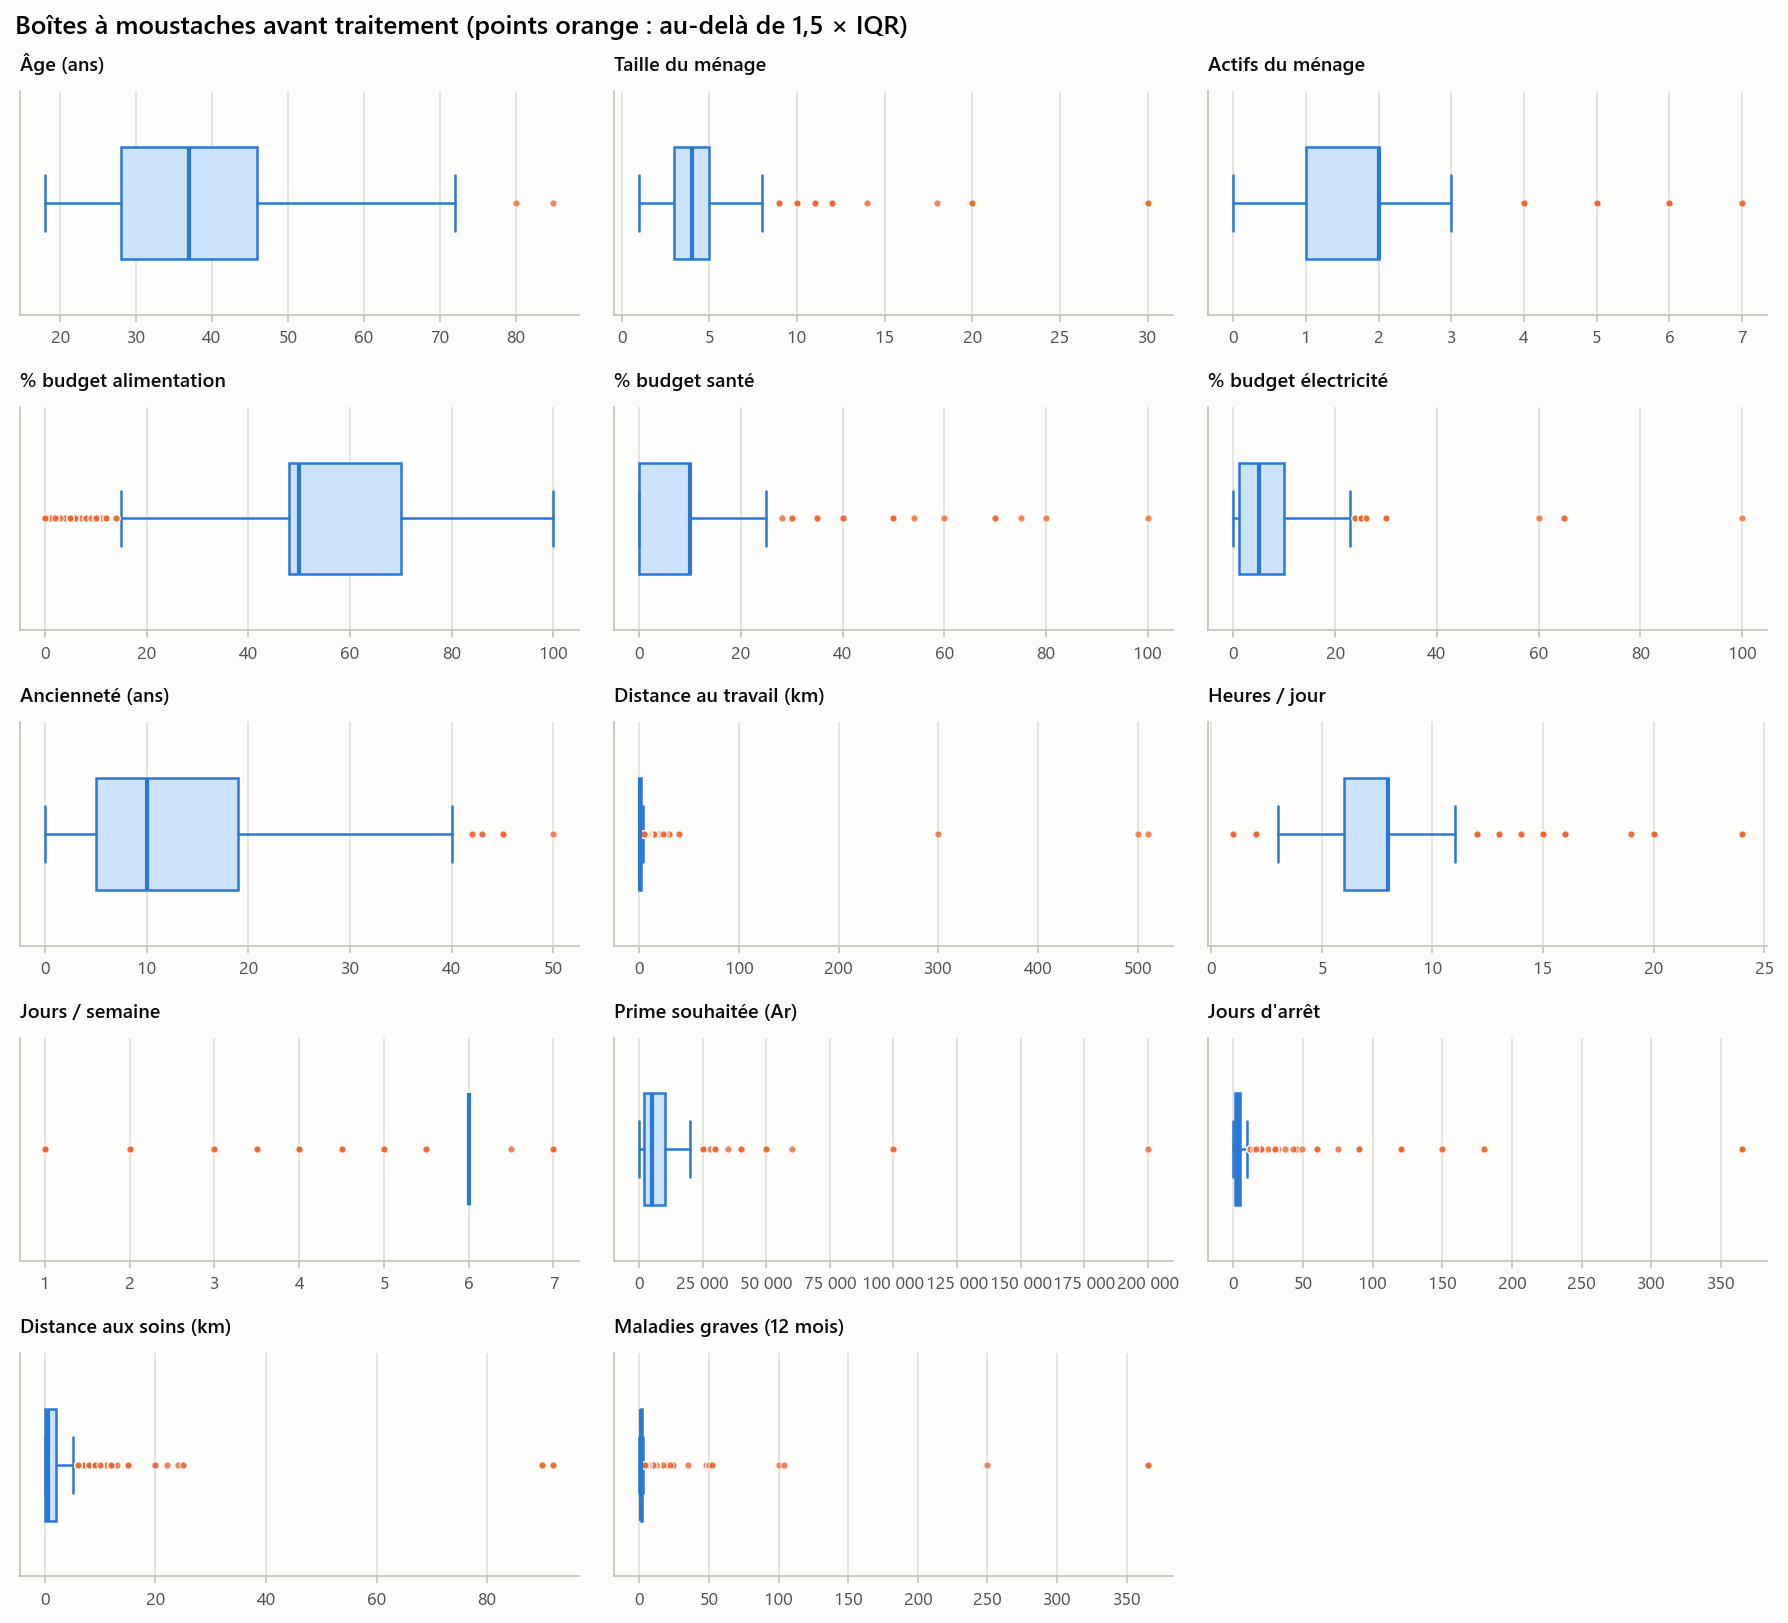
\includegraphics[keepaspectratio,alt={Boîtes à moustaches}]{resultats/figures/boites_avant_traitement.png}}

\caption{Boîtes à moustaches}

\end{figure}



\begin{figure}

\centering

\pandocbounded{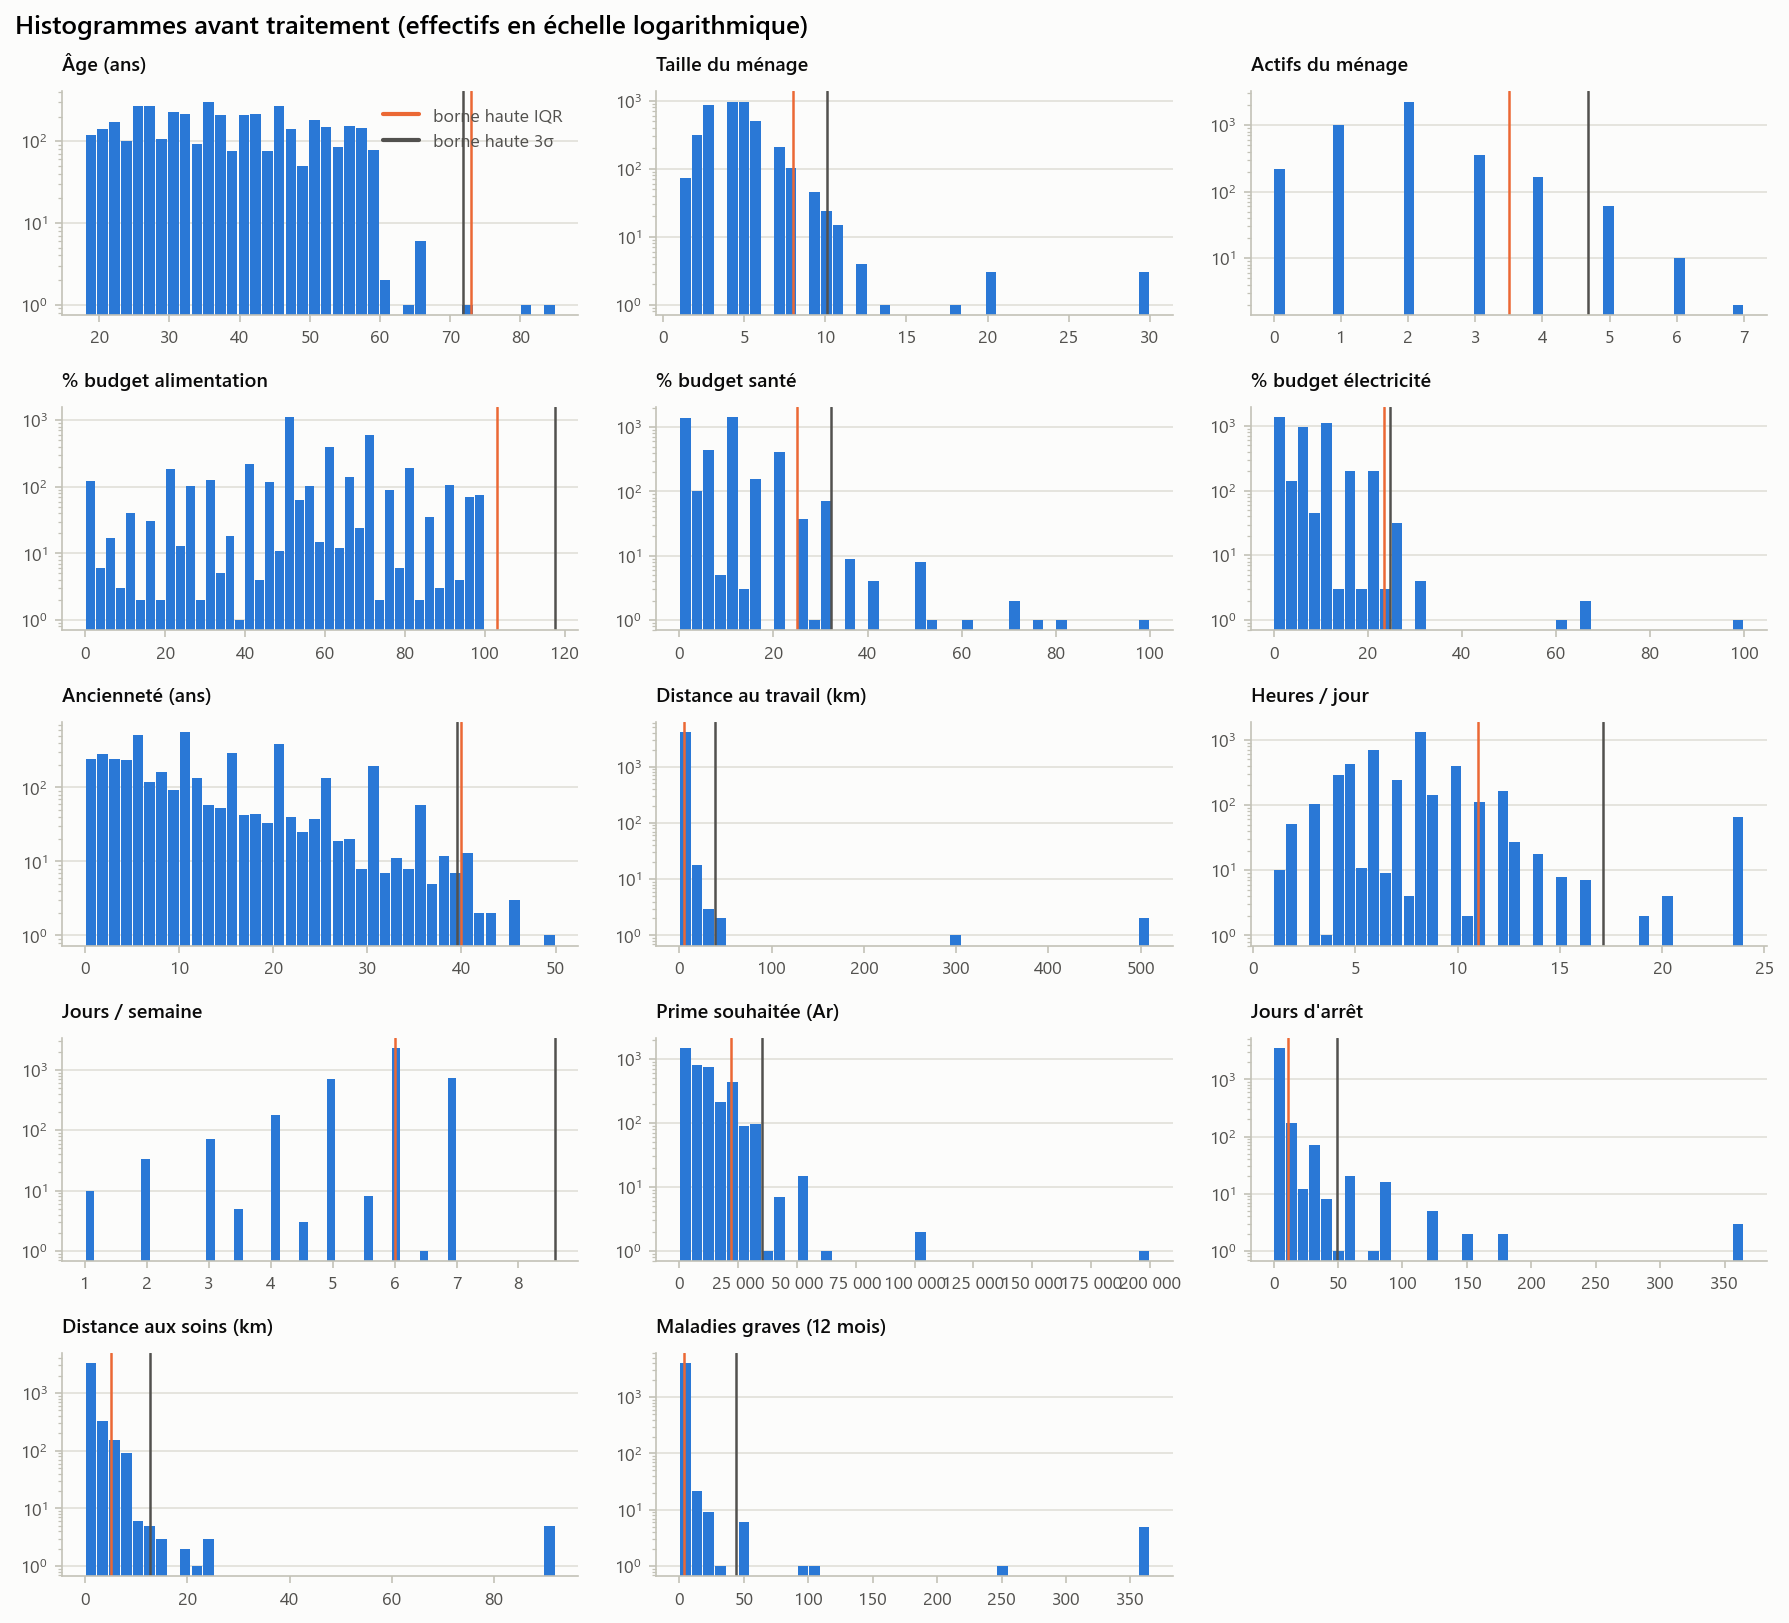
\includegraphics[keepaspectratio,alt={Histogrammes}]{resultats/figures/histogrammes_avant_traitement.png}}

\caption{Histogrammes}

\end{figure}



\section{2. Variable de fréquence : choix du seuil}



\begin{figure}

\centering

\pandocbounded{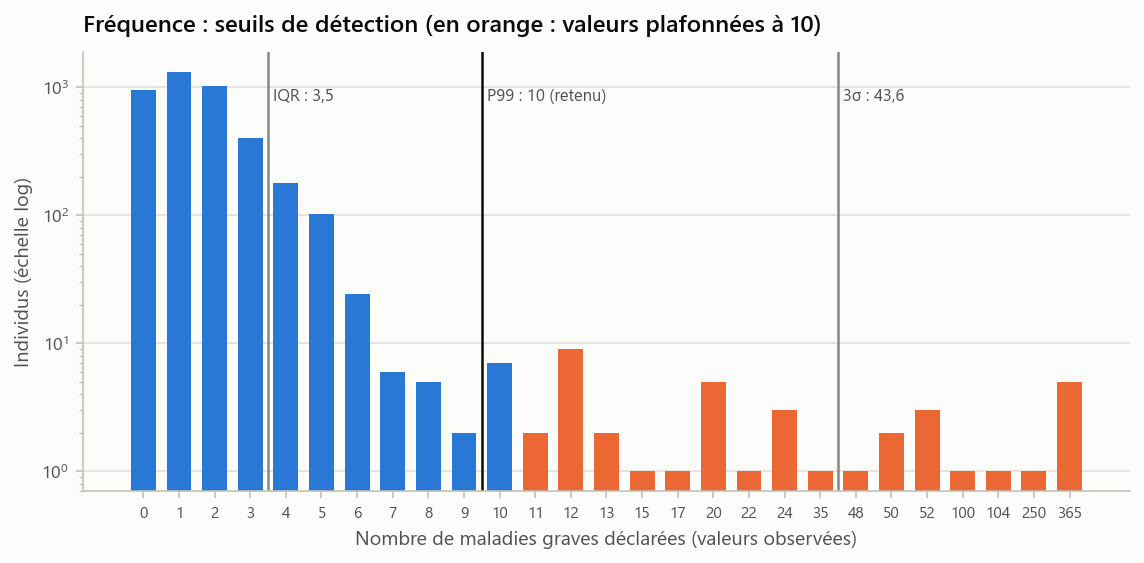
\includegraphics[keepaspectratio,alt={Seuils pour la fréquence}]{resultats/figures/seuils_frequence.png}}

\caption{Seuils pour la fréquence}

\end{figure}



La décroissance de 0 à 10 maladies est régulière : ce sont des comptages plausibles. Au-delà de 10, les valeurs (12, 20, 24, 52, 100, 365) correspondent visiblement à un nombre de mois, de semaines ou de jours de maladie, c'est-à-dire aux crises répétées d'une même maladie chronique et non à des sinistres distincts. \textbf{On plafonne donc au 99e centile (10)} :



{\def\LTcaptype{none} % do not increment counter

\begin{longtable}[]{@{}lrr@{}}

\toprule\noalign{}

& Avant & Après \\

\midrule\noalign{}

\endhead

\bottomrule\noalign{}

\endlastfoot

Moyenne & 2,25 & \textbf{1,61} \\

Variance & 190,1 & \textbf{2,53} \\

Variance / moyenne & 84,5 & \textbf{1,58} \\

Maximum & 365 & 10 \\

Valeurs modifiées & --- & 39 (0,96 \%) \\

\end{longtable}

}



Le plafonnement ne touche que 1 \% des individus mais ramène la variance de 190 à 2,5. Le rapport variance / moyenne de 1,58 reste supérieur à 1, signe d'une \textbf{surdispersion modérée} qui sera testée à l'étape 3.1 (Poisson ou binomiale négative). Le choix du seuil a peu d'effet : seules 13 valeurs se situent entre 11 et 13.



\section{3. Variable de sévérité : écrêtement}



\begin{figure}

\centering

\pandocbounded{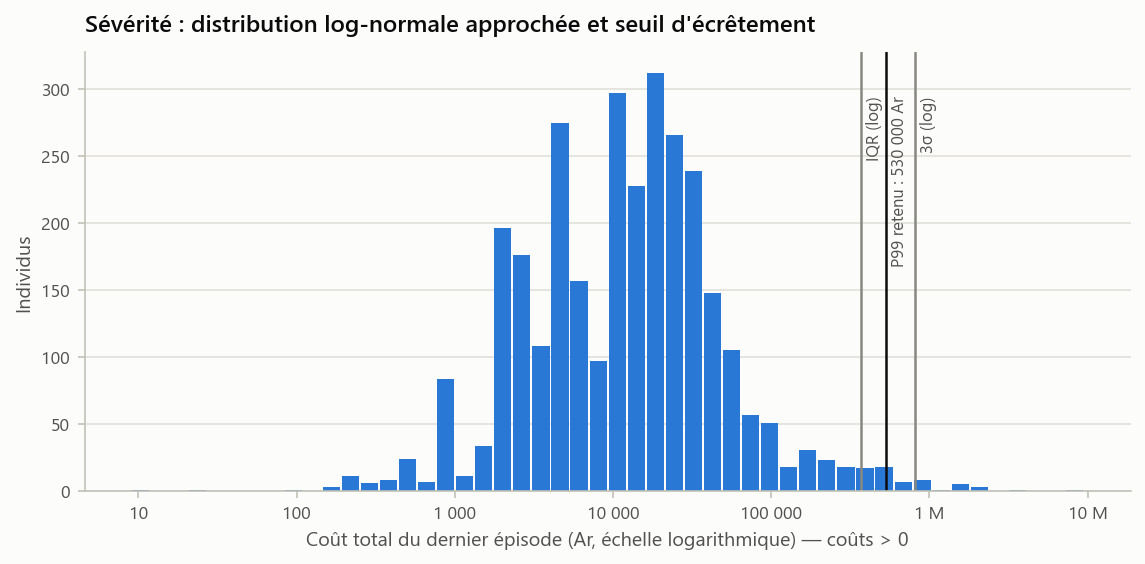
\includegraphics[keepaspectratio,alt={Seuils pour le coût}]{resultats/figures/seuils_cout.png}}

\caption{Seuils pour le coût}

\end{figure}



Sur l'échelle logarithmique, le coût suit approximativement une loi log-normale (une légère bimodalité vient des montants ronds : 2 000, 5 000, 10 000, 20 000 Ar). Les plus gros coûts (hospitalisation de 7 M Ar, scanner de 2,4 M Ar, chimiothérapie de 2 M Ar) sont \textbf{réels} : les supprimer ferait disparaître le risque que l'assurance doit couvrir. On applique la méthode actuarielle de l'\textbf{écrêtement} :



\begin{enumerate}

\def\labelenumi{\arabic{enumi}.}

\tightlist

\item

  le coût est plafonné au \textbf{99e centile des coûts positifs : 530 000 Ar} (30 valeurs) pour estimer le GLM de sévérité, qui serait sinon dominé par une poignée de sinistres ;

\item

  la charge au-delà du seuil n'est pas perdue : elle est \textbf{redistribuée sur toutes les primes} à l'étape 3.3 par un coefficient de chargement ;

\item

  le coût brut reste disponible dans \texttt{cout\_total\_brut}.

\end{enumerate}



{\def\LTcaptype{none} % do not increment counter

\begin{longtable}[]{@{}lrr@{}}

\toprule\noalign{}

Coûts positifs (3 054 individus) & Avant & Après écrêtement \\

\midrule\noalign{}

\endhead

\bottomrule\noalign{}

\endlastfoot

Moyenne (Ar) & 41 191 & 32 683 \\

Médiane (Ar) & 13 005 & 13 005 \\

Coefficient de variation & 5,29 & \textbf{2,28} \\

Maximum (Ar) & 9 500 000 & 530 000 \\

Part de la charge totale au-delà du seuil & --- & \textbf{20,6 \%} \\

\end{longtable}

}



Le 1 \% de sinistres les plus graves représente un cinquième de la charge totale : c'est la signature d'un risque santé à queue épaisse, qui justifie le mécanisme d'écrêtement et de redistribution.



\section{4. Stratégie retenue pour chaque variable}



{\def\LTcaptype{none} % do not increment counter

\begin{longtable}[]{@{}

  >{\raggedright\arraybackslash}p{(\linewidth - 10\tabcolsep) * \real{0.1667}}

  >{\raggedright\arraybackslash}p{(\linewidth - 10\tabcolsep) * \real{0.1667}}

  >{\raggedright\arraybackslash}p{(\linewidth - 10\tabcolsep) * \real{0.1667}}

  >{\raggedleft\arraybackslash}p{(\linewidth - 10\tabcolsep) * \real{0.1667}}

  >{\raggedleft\arraybackslash}p{(\linewidth - 10\tabcolsep) * \real{0.1667}}

  >{\raggedright\arraybackslash}p{(\linewidth - 10\tabcolsep) * \real{0.1667}}@{}}

\toprule\noalign{}

\begin{minipage}[b]{\linewidth}\raggedright

Variable

\end{minipage} & \begin{minipage}[b]{\linewidth}\raggedright

Rôle

\end{minipage} & \begin{minipage}[b]{\linewidth}\raggedright

Traitement

\end{minipage} & \begin{minipage}[b]{\linewidth}\raggedleft

Seuil

\end{minipage} & \begin{minipage}[b]{\linewidth}\raggedleft

Valeurs modifiées

\end{minipage} & \begin{minipage}[b]{\linewidth}\raggedright

Justification

\end{minipage} \\

\midrule\noalign{}

\endhead

\bottomrule\noalign{}

\endlastfoot

age & explicative & \textbf{Conservation} & --- & 0 & Après l'étape 1.1, l'âge va de 18 à 85 ans ; les âges de 80 à 85 ans sont réels et rares \\

taille\_menage & explicative & \textbf{Plafonnement P99} & 10 & 27 & Les grandes familles existent, mais 20 ou 30 personnes relèvent d'un foyer collectif ; le plafond limite leur poids dans les distances du K-means \\

nb\_actifs\_menage & explicative & \textbf{Conservation} & --- & 0 & Valeurs de 0 à 7, toutes plausibles \\

budget\_alim & explicative & \textbf{Conservation} & --- & 0 & Bornée à {[}0 ; 100{]} \% depuis l'étape 1.1 \\

budget\_sante & explicative & \textbf{Plafonnement P99} & 30 \% & 28 & Distribution très asymétrique ; 50 à 100 \% pèsent trop dans les distances \\

budget\_elec & explicative & \textbf{Plafonnement P99} & 24 \% & 40 & Même raison \\

anciennete\_emploi & explicative & \textbf{Conservation} & --- & 0 & Déjà limitée par l'âge (\ensuremath{\leq} âge \ensuremath{-} 5) à l'étape 1.1 \\

distance\_travail & explicative & \textbf{Plafonnement P99} & 10 km & 34 & Queue extrême (300 et 510 km) issue de saisies ambiguës \\

heures\_jour & explicative & \textbf{Plafonnement à 16 h} & 16 h & 71 & « 24 h » ou « 24/24 » décrit un temps de présence, pas un travail effectif ; 16 h est proche de la borne des 3\ensuremath{\sigma} (17,1) \\

jours\_semaine & explicative & \textbf{Conservation} & --- & 0 & Bornée à {[}1 ; 7{]} ; l'IQR nul n'est pas pertinent \\

\textbf{nb\_maladies\_graves} & cible & \textbf{Plafonnement P99} & 10 & 39 & Voir \S{} 2 \\

\textbf{cout\_total} & cible & \textbf{Écrêtement P99} + redistribution & 530 000 Ar & 30 & Voir \S{} 3 \\

prime\_souhaitee & descriptive & Plafonnement P99 & 30 000 Ar & 27 & Évite qu'une réponse isolée (200 000 Ar) fausse les moyennes \\

jours\_arret & descriptive & Plafonnement P99 & 60 j & 29 & Arrêts de plusieurs mois réels mais rares \\

distance\_soins & descriptive & Plafonnement P99 & 9 km & 25 & Soins pris à Antananarivo ou Antsirabe (90 km et plus) \\

\end{longtable}

}



\textbf{Pourquoi plafonner plutôt que supprimer ?} Supprimer une ligne fait perdre les 58 autres informations de l'individu, et supprimer les gros sinistres sous-estimerait le risque. Le plafonnement (winsorisation) garde l'individu, conserve l'ordre des valeurs (un extrême reste au sommet de la distribution) et ne modifie que 0,7 à 1,7 \% des valeurs de chaque variable traitée.



\textbf{Transformation} : la transformation logarithmique sert à la \textbf{détection} pour les coûts. Pour la \textbf{modélisation}, la loi de la sévérité (Gamma ou log-normale) est choisie à l'étape 3.2 : le GLM Gamma à lien log tient déjà compte de l'asymétrie.



\begin{figure}

\centering

\pandocbounded{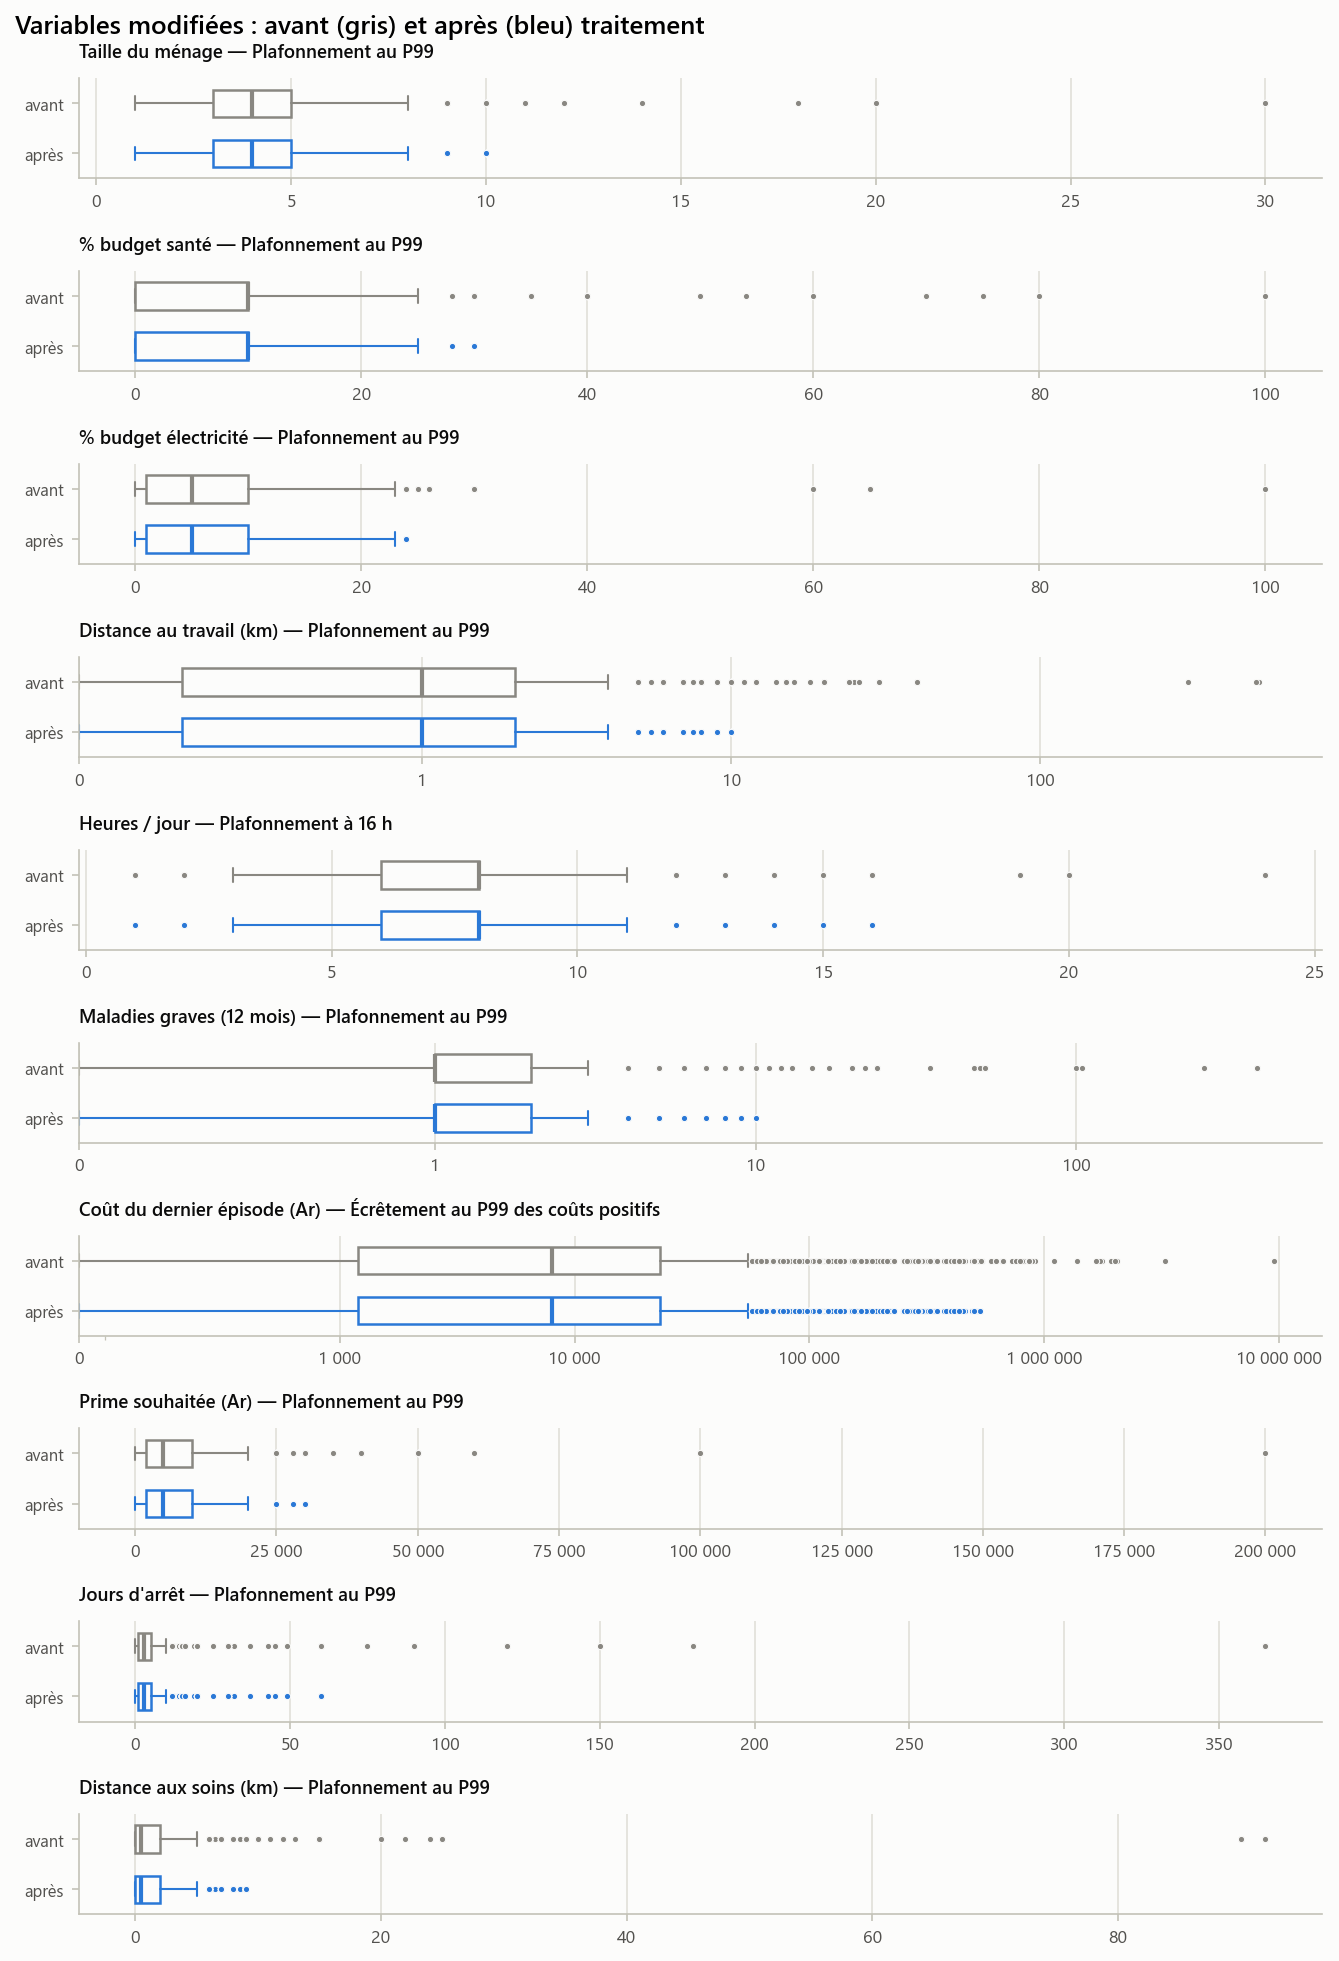
\includegraphics[keepaspectratio,alt={Avant / après traitement}]{resultats/figures/avant_apres_traitement.png}}

\caption{Avant / après traitement}

\end{figure}



\section{5. Populations pour la modélisation (calculées sur le jeu traité)}



{\def\LTcaptype{none} % do not increment counter

\begin{longtable}[]{@{}

  >{\raggedright\arraybackslash}p{(\linewidth - 4\tabcolsep) * \real{0.3333}}

  >{\raggedleft\arraybackslash}p{(\linewidth - 4\tabcolsep) * \real{0.3333}}

  >{\raggedright\arraybackslash}p{(\linewidth - 4\tabcolsep) * \real{0.3333}}@{}}

\toprule\noalign{}

\begin{minipage}[b]{\linewidth}\raggedright

Population

\end{minipage} & \begin{minipage}[b]{\linewidth}\raggedleft

Effectif

\end{minipage} & \begin{minipage}[b]{\linewidth}\raggedright

Usage

\end{minipage} \\

\midrule\noalign{}

\endhead

\bottomrule\noalign{}

\endlastfoot

Tous les individus & 4 074 & Segmentation K-means, CART \\

Nombre de maladies graves renseigné & 4 046 & GLM de fréquence (étape 3.1) \\

Au moins un sinistre (\emph{N} \ensuremath{\geq} 1) & 3 103 & --- \\

\ldots{} dont coût positif & \textbf{2 555} & \textbf{GLM de sévérité} (étape 3.2) \\

\ldots{} dont coût nul (remède traditionnel, aucun recours) & 486 (16 \% des sinistres renseignés) & Pris en compte dans la prime pure (étape 3.3) \\

\ldots{} dont coût manquant & 62 & Exclus du GLM de sévérité \\

\end{longtable}

}



Dans la population de sévérité, le rapport entre la charge brute et la charge écrêtée vaut \textbf{1,289} : c'est le coefficient de redistribution de l'écrêtement utilisé à l'étape 3.3.



\ensuremath{\rightarrow} Suite : \href{../1.3_preparation/README.pdf}{étape 1.3 --- Préparation pour la modélisation}



\section{Fichiers produits}



{\def\LTcaptype{none} % do not increment counter

\begin{longtable}[]{@{}

  >{\raggedright\arraybackslash}p{(\linewidth - 2\tabcolsep) * \real{0.5000}}

  >{\raggedright\arraybackslash}p{(\linewidth - 2\tabcolsep) * \real{0.5000}}@{}}

\toprule\noalign{}

\begin{minipage}[b]{\linewidth}\raggedright

Fichier

\end{minipage} & \begin{minipage}[b]{\linewidth}\raggedright

Contenu

\end{minipage} \\

\midrule\noalign{}

\endhead

\bottomrule\noalign{}

\endlastfoot

\texttt{resultats/donnees\_sans\_aberrantes.csv} / \texttt{.xlsx} & \textbf{Jeu traité} (entrée de l'étape 1.3) \\

\texttt{tables/detection\_aberrantes.csv} & Statistiques, bornes IQR et 3\ensuremath{\sigma}, effectifs hors bornes pour chaque variable \\

\texttt{tables/traitement\_aberrantes.csv} & Stratégie, seuil, valeurs modifiées et justification \\

\texttt{tables/effet\_frequence.csv}, \texttt{effet\_cout.csv} & Effet du traitement sur les deux cibles \\

\texttt{figures/boites\_avant\_traitement.png}, \texttt{histogrammes\_avant\_traitement.png} & Détection graphique \\

\texttt{figures/seuils\_frequence.png}, \texttt{seuils\_cout.png} & Choix des seuils pour les cibles \\

\texttt{figures/avant\_apres\_traitement.png} & Variables modifiées, avant et après \\

\texttt{resultats/journal.txt} & Sortie complète du script \\

\end{longtable}

}



\end{document}

